\chap{Results}
In this chapter, the most important findings from the four studies will be highlighted. For the full results, see the individual studies.

\sect{Study I}
Study I was a proof-of-concept study to determine if a golden-angle based imaging approach could improve imaging of the pulmonary vasculature, in the context of imaging diagnosis of pulmonary embolism. Diagnosis using MRI had previously been suggested~\cite{Stein2010, Kalb2012, Revel2013}, and in this study, the novel method was compared to a Cartesian free-breathing protocol with multiple repetitions~\cite{Nyren2017}. A number of encoding ordering strategies were tested, i.e. linear ordering, centric ordering, and golden-angle ordering. It was shown that the linear ordering caused the highest degree of image artifacts. The centric ordering scheme somewhat reduced the artifacts, but there was still a severe artifact obscuring the anatomy. Using the golden-angle profile ordering, the artifacts disappeared almost entirely. See figure~\ref{fig:study1_2}.
\begin{figure}[htbp]
    \centering
    \includegraphics[width=\textwidth]{kspace_ordering}
    \caption{Different k-space orderings and corresponding image quality. Conventional linear ordering shows the highest amount of image artifacts (left), whereas the artifacts are slightly reduced with a centric ordering (middle). Using a golden-angle ordering, there are very little image artifacts present (right). Reproduced with permission from~\cite{Fyrdahl2018}. Copyright \copyright~2018 International Society for Magnetic Resonance in Medicine. Published by John Wiley \& Sons Inc.}
    \label{fig:study1_2}
\end{figure}
The golden-angle approach was evaluated using a sliding-window approach in two patients. A large thrombus was visible in the left pulmonary artery in both subjects. However, there is a clear difference in image quality between the Cartesian and golden-angle acquisitions. To quantify the difference in visibility, the blood-to-blood-clot-contrast was calculated and found to be 23\% higher for the golden-angle acquisition in both cases.
\begin{figure}[htbp]
    \centering
    \includegraphics[width=\textwidth]{patients}
    \caption{Representative examples in two different patients with confirmed pulmonary embolism. Cartesian images show a moderate amount of artifacts (left), whereas the golden-angle radial acquisition has less image artifacts (right). The white arrows indicate a thrombus. Reproduced with permission from~\cite{Fyrdahl2018}. Copyright \copyright~2018 International Society for Magnetic Resonance in Medicine. Published by John Wiley \& Sons Inc.}
    \label{fig:study1_3}
\end{figure}
Two experienced observers were asked to score the image quality for the Cartesian and the golden-angle acquisition using three different temporal footprints. The results of the scoring are presented in Table~\ref{table:study1scores}.
\begin{table}[htbp]
\caption{Summary of observer scores for both Cartesian and golden-angle radial, with 144, 610 and 1345 spokes.}
\begin{center}
\begin{threeparttable}
\begin{tabular}{l c c c c}
     \mydarkrowcolor~ & Cartesian & \multicolumn{3}{c}{Golden Angle} \\
     \mydarkrowcolor~ & ~ & 144 spokes & 610 spokes & 1345 spokes \\
     Diagnostic quality & $2.2 \pm 0.6$ & $2.3 \pm 0.7$ & $2.8 \pm 0.8$ & $3.5 \pm 0.9$ \\
     \myrowcolor Vessel sharpness & $2.1 \pm 0.5$ & $2.2 \pm 0.8$ & $2.6 \pm 0.9$ & $3.4 \pm 0.9$ \\
     Artifacts & $3.0 \pm 1.0$ & $3.0 \pm 0.9$ & $3.4 \pm 0.8$ & $3.9 \pm 0.7$ \\
     \bottomrule
\end{tabular}
\begin{tablenotes}
\emph{Note:} Continuous values are presented as mean $\pm$ SD. Higher scores means better images.
\end{tablenotes}
\end{threeparttable}
\end{center}
\label{table:study1scores}
\end{table}

\sect{Study II}
In study II, a modified 3D-radial double golden angle profile ordering was proposed to reduce eddy current artifacts. The proposed profile orderings showed a uniform behavior, in comparison to a completely random profile ordering, see Figure~\ref{fig:study2_1}, which was also confirmed by numerical calculations of the CCR-continuum.
\begin{figure}[htbp]
    \centering
    \includegraphics[width=\textwidth]{fig_1_trajectories.png}
    \caption{A completely random profile ordering (black box) compared to the original double golden angle profile ordering as well as Tiny 5, 8, 13, 21, 34 and 55. There is an apparent uniformity to the golden, and tiny profile orderings, which is not present in the random distribution. This finding is corroborated by the CRR measure.}
    \label{fig:study2_1}
\end{figure}
One profile ordering, Tiny-13, was chosen for further testing. It was compared to the original double golden angle profile ordering~\cite{Chan2009}, by performing a simulated physiological binning based on pre-recorded ECG and respiratory signals. Binning was performed into 20 and 25 cardiac phases as well as 2, 4 and 6 respiratory bins. The profile ordering was calculated for all time frames for both profile orderings. Tiny-13 showed a higher degree of k-space uniformity in all cases except for 25 cardiac phases and 6 respiratory bins, where differences did not reach statistical significance.
\begin{figure}[htbp]
    \centering
    \includegraphics[width=\textwidth]{phantom_modified.png}
    \caption{Phantom acquisitions of the original double golden angle profile ordering and Tiny 5, 8, 13, 21, 34 and 55 (from left to right). There is a gradual decrease in image artifacts with a decreasing angle between successive readouts.}
    \label{fig:study2_2}
\end{figure}
\begin{figure}[htbp]
    \centering
    \includegraphics[width=\textwidth]{in_vivo_modified_lighter.png}
    \caption{\emph{In vivo} measurements in a healthy volunteer with the original double golden angle profile ordering (left) and the proposed Tiny-13 profile ordering (right) show a maintained ability to perform physiological binning, and an improvement in the image homogeneity with the reduced angular step.}
    \label{fig:study2_3}
\end{figure}
\sect{Study III}
In Study III, a modified golden-angle phase contrast pulse sequence was proposed and evaluated for measurements of transmitral blood-flow and tissue velocities in patients. The PSF-analysis showed a higher sampling uniformity, and subsequently a lower peak PSF as a function of radius for the SWIG method compared to conventional golden-angle, see Figure~\ref{fig:study3_1}.

\begin{figure}[htbp]
    \centering
    \includegraphics[width=\textwidth]{Figure_2_PSF}
    \caption{Examples of the k-space sampling distribution and the corresponding PSF for both SWIG and the conventional golden-angle profile ordering (A). The peak PSF and PSF energy as a function of radius (B). Reproduced from~\cite{Fyrdahl2020}. (Licensed under CC-BY-4.0)}
    \label{fig:study3_1}
\end{figure}

The pilot study showed that depending on the temporal footprint selected, CMR could either underestimate or overestimate the velocities compared to tissue Doppler echocardiography, see Figure~\ref{fig:study3_abstract}. It was clear that a smaller temporal footprint produced a sharper velocity peak, however, at the expense of increased noise, see Figure~\ref{fig:study3_2}. For a summary of the results from the pilot study, see Table~\ref{table:study3footprint}.

\begin{figure}[htbp]
    \centering
    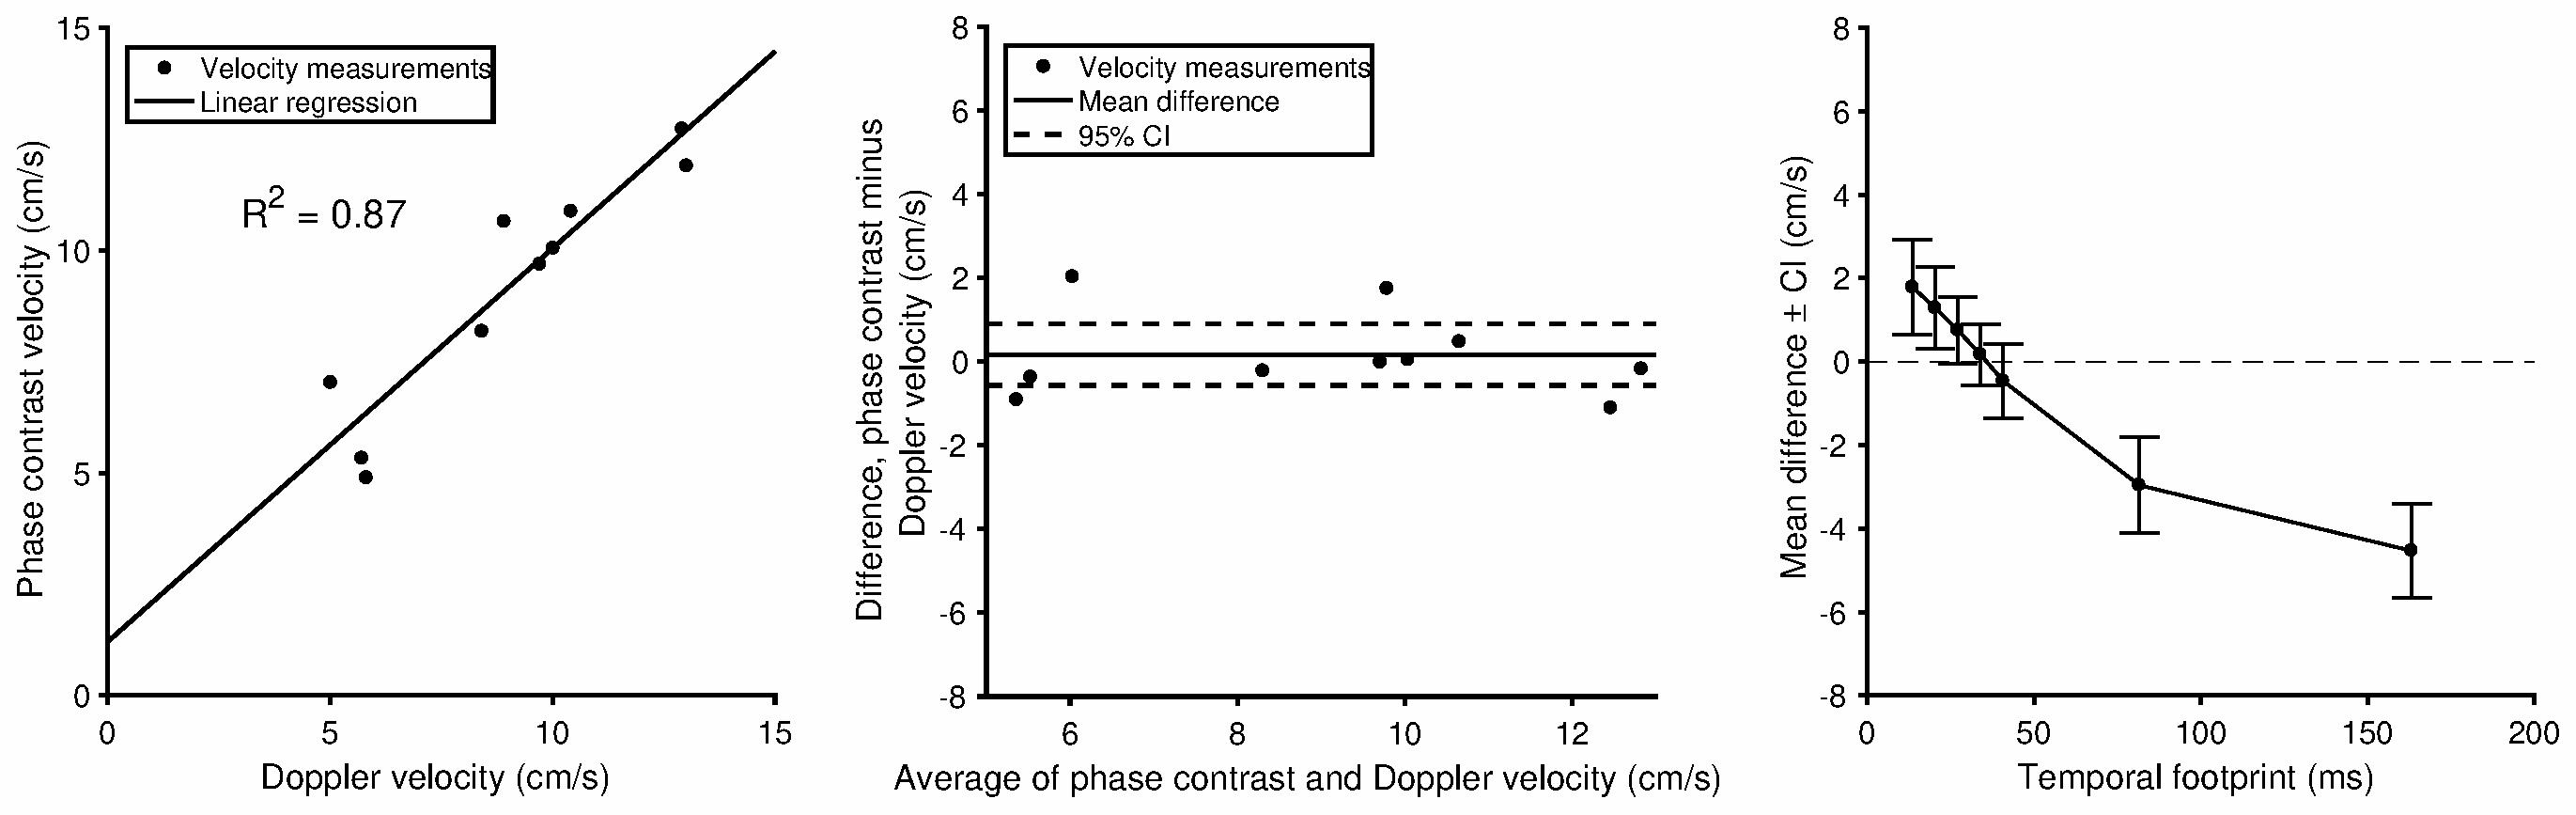
\includegraphics[width=\textwidth]{corr_6}
    \caption{Results from the pilot study. The correlation is shown for a temporal footprint for CMR of 34 ms (left) with corresponding Bland-Altman plot (middle). A temporal footprint between 27.2 ms and 40.8 ms did not differ when compared between CMR and tissue Doppler. Using larger footprints for CMR resulted in an apparent underestimation, whereas using a smaller temporal footprint resulted in an apparent overestimation of the tissues velocities compared to tissue Doppler (right). Reproduced from~\cite{Fyrdahl2018:SCMR}.}
    \label{fig:study3_abstract}
\end{figure}


\begin{figure}[htbp]
    \centering
    \includegraphics[width=\textwidth]{Figure_3_Multiple_resolutions}
    \caption{Representative phase contrast images in systole, early filling and late filling (A). Time velocity curves measured in a single voxel in the lateral wall. Different colors represents different temporal footprints. The black box indicates the early filling velocity peak (B). A magnified view of the early filling peak (C). Reproduced from~\cite{Fyrdahl2020}. (Licensed under CC-BY-4.0)}
    \label{fig:study3_2}
\end{figure}

\begin{table}[htbp]
\caption{Comparison between CMR-derived and Doppler-derived myocardial velocities in early filling (e') with a variable temporal footprint and a fixed temporal increment.}
\begin{center}
\begin{threeparttable}
\begin{tabular}{c c c c c c c}
     \mydarkrowcolor \multicolumn{3}{c}{\textbf{Temporal footprint}} & \textbf{Correlation} & \textbf{Mean difference} & \textbf{95\% LoA} & \textbf{P} \\
     \mydarkrowcolor \quad & (TR) & (ms) & (R$^2$) & (cm/s) & (cm/s) & ~\\
     \quad & 4 & 27.2 & 0.46 & 1.0 & 4.3 & 0.03 \\
     \myrowcolor \quad & 6 & 40.8 & 0.63 & 0.9 & 3.4 & 0.13 \\
     \quad & 8 & 54.5 & 0.72 & 0.4 & 3.0 & 0.41 \\
     \myrowcolor \quad & 10 & 68.0 & 0.69 & -0.2 & 3.3 & 0.71 \\
     \quad & 12 & 81.6 & 0.65 & -0.9 & 3.5 & 0.14 \\
     \bottomrule
\end{tabular}
\begin{tablenotes}
\emph{Note:} P-values denote outcome of Mann-Whitney U-test with the null hypothesis that the CMR and Doppler velocities did not differ. LoA – Limits of Agreement.\\
\end{tablenotes}
\end{threeparttable}
\end{center}
\label{table:study3footprint}
\end{table}

The patient study showed a high degree of correlation for measurement of tissue velocities but a systematic underestimation of transmitral blood flow velocities, see Figure~\ref{fig:study3_3}. For a summary of all results from the patient study, see Table~\ref{table:study3summary}.

\begin{figure}[htbp]
    \centering
    \includegraphics[width=\textwidth]{Figure_5_Myo+Mitral}
    \caption{Scatter plot (A) and the corresponding Bland-Altman plot (B) for myocardial tissue velocities (s’, e’, a’) measured separately in the septal and lateral wall with both tissue Doppler echocardiography and phase contrast CMR. Scatter plot (C) and the corresponding Bland-Altman plot (D) for peak transmitral velocities (E, A) measured with both Doppler echocardiography and phase contrast CMR. Reproduced from~\cite{Fyrdahl2020}. (Licensed under CC-BY-4.0)}
    \label{fig:study3_3}
\end{figure}

\begin{table}[htbp]
\caption{Comparison between CMR-derived and Doppler-derived myocardial velocities in early filling (e') with a variable temporal footprint and a fixed temporal increment.}
\begin{center}
\begin{threeparttable}
\begin{tabular}{c c c c c c c}
     \mydarkrowcolor \multicolumn{7}{l}{\textbf{Myocardial velocity}} \\
     \mydarkrowcolor ~ & \textbf{Doppler} & \textbf{CMR} & \textbf{P} & \textbf{Correlation} & \textbf{Mean diff.} & \textbf{95\% LoA} \\
     \mydarkrowcolor ~ & (cm/s) & (cm/s) & ~ & (R$^2$) & (cm/s) & (cm/s) \\ 
     All & $8.2 \pm 3.0$ & $9.0 \pm 3.0$ & $<0.005$ & $0.63$ & $0.9$ & $\pm 3.7$ \\
     \myrowcolor s' & $7.1 \pm 1.8$ & $8.1 \pm 2.1$ & $<0.005$ & $0.34$ & $1.0$ & $\pm 3.4$ \\
     e' & $8.1 \pm 2.7$ & $9.1 \pm 3.1$ & $<0.005$ & $0.74$ & $0.8$ & $\pm 3.5$ \\
     \myrowcolor a' & $9.4 \pm 3.5$ & $10.2 \pm 3.3$ & $< 0.005$ & $0.54$ & $1.0$ & $\pm 4.2$ \\
     \mydarkrowcolor \multicolumn{7}{l}{\textbf{Transmitral blood flow velocity}} \\
     \mydarkrowcolor ~ & \textbf{Doppler} & \textbf{CMR} & \textbf{P} & \textbf{Correlation} & \textbf{Mean diff.} & \textbf{95\% LoA} \\
     \mydarkrowcolor ~ & (cm/s) & (cm/s) & ~ & (R$^2$) & (cm/s) & (cm/s) \\
    All & $67 \pm 18$ & $56 \pm 16$ & $<0.005$ & $0.45$ & $-11$ & $\pm 28$ \\
    \myrowcolor E & $74 \pm 17$ & $60 \pm 15$ & $<0.005$ & $0.27$ & $-14$ & $\pm 31$ \\
    A & $60 \pm 17$ & $51 \pm 17$ & $<0.005$ & $0.53$ & $-8$ & $\pm 25$ \\
    \mydarkrowcolor \multicolumn{7}{l}{\textbf{Derived parameters}} \\
     \mydarkrowcolor ~ & \textbf{Doppler} & \textbf{CMR} & \textbf{P} & \textbf{Correlation} & \textbf{Mean diff.} & \textbf{95\% LoA} \\
     \mydarkrowcolor ~ & (a.u) & (a.u) & ~ & (R$^2$) & (a.u.) & (a.u.) \\ 
    E/e'& $8.58 \pm 3.28$ & $6.25 \pm 2.28$ & $<0.005$ & $0.34$ & $-2.3$ & $\pm 5.3$ \\
    \myrowcolor E/A & $1.34 \pm 0.50$ & $1.31 \pm 0.55$ & $0.295$ & $0.66$ & $0.03$ & $\pm 0.6$ \\
\end{tabular}
\begin{tablenotes}
\emph{Note:} Continuous values are presented as mean $\pm$ SD. P-values denote outcome of Mann-Whitney U-test with the null hypothesis that the CMR and Doppler velocities did not differ. LoA – Limits of Agreement.\\
\end{tablenotes}
\end{threeparttable}
\end{center}
\label{table:study3summary}
\end{table}

\sect{Study IV}
The result from the PSF-analysis showed that for high undersampling factors, i.e., 12 patches, there was a clear difference in the PSF between the double golden-angle profile ordering and the 3D-SWIG profile ordering. For 48 patches and 192 patches (R=1), the difference was less prominent, albeit with a slight edge to the 3D-SWIG profile ordering, see Figure~\ref{fig:study4_1}. For the three subjects, the k-space uniformity was significantly higher for SWIG-3D compared to the double golden-angle profile ordering, see Figure~\ref{fig:study4_2}.
\begin{figure}[htbp]
    \centering
    \includegraphics[width=\textwidth]{Fig5_PSF}
    \caption{Examples of the PSF for both 3D-SWIG and the conventional double golden-angle profile ordering for 12, 48 and 192 sectors (left). The aliasing a function of radius show a difference for 12 sectors, but a decreasing difference as the number of sectors is increased.}
    \label{fig:study4_1}
\end{figure}
\begin{figure}[htbp]
    \centering
    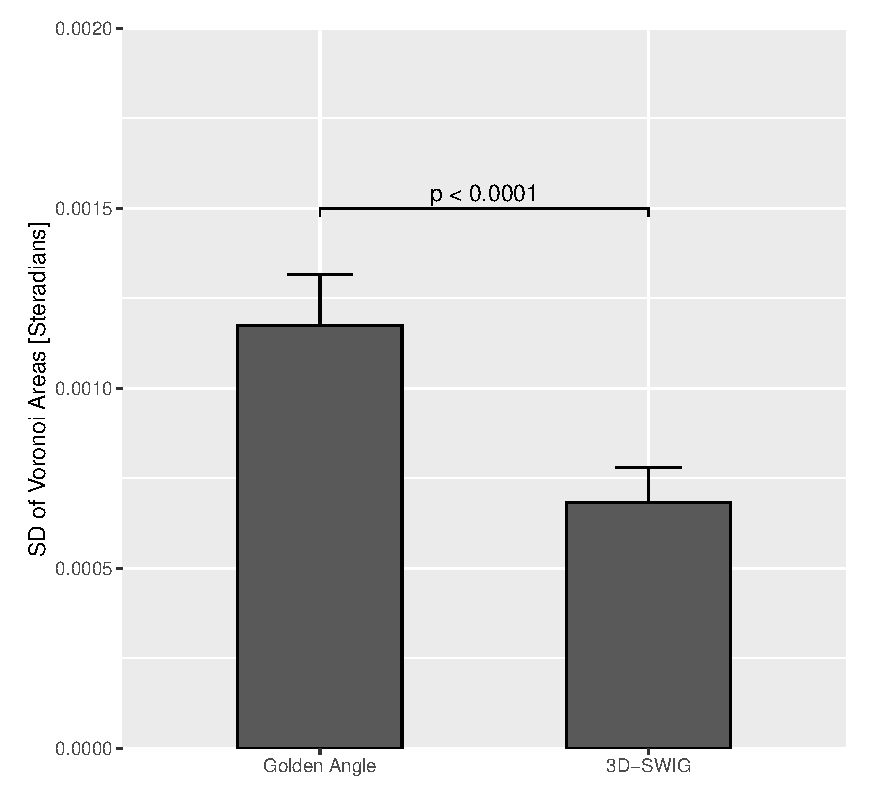
\includegraphics[width=0.75\textwidth]{Rplot02}
    \caption{The standard deviation of Voronoi cell areas was used to assess k-space uniformity after binning. The data from the three subjects were reconstructed into 20 cardiac bins and 3 respiratory bins, resulting in a total of 180 bins, and all Voronoi cell areas were calculated for each bin. A lower value indicates a more uniform k-space.}
    \label{fig:study4_2}
\end{figure}

